\documentclass[10pt,a4paper]{book}
\usepackage[utf8]{inputenc}
\usepackage[spanish]{babel}
\usepackage{amsmath}
\usepackage{amsfonts}
\usepackage{amssymb}
\usepackage{graphicx}
\usepackage{xymtex}
\author{\underline {César} Lozano}
\title{Ejercicio de \LaTeX}

%lista, imagen, ecuación, tabla

\begin{document}


\begin{titlepage}
\begin{Huge}
\maketitle
\end{Huge}
\end{titlepage}
\thispagestyle{empty}
$\ $


\tableofcontents
\pagenumbering{arabic}
\chapter{Lista}
\section{Tabla 1}
\begin{enumerate}
\item Ítem 1
\item Ítem 2
\item Ítem 3
\end{enumerate}
\section{Tabla 2}
\begin{flushright}
\begin{itemize}
\item Ítem A
\item Ítem C\footnote{Me he saltado el Ítem B...}
\end{itemize}
\end{flushright}


\cleardoublepage


\chapter{Imagen}
\begin{figure}[hbt]
\begin{center}
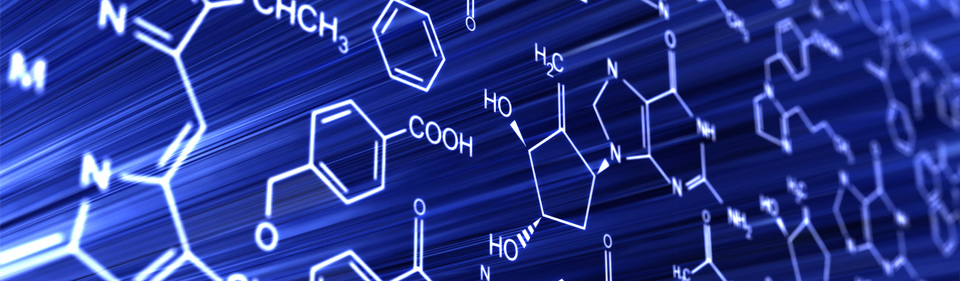
\includegraphics[scale=0.3]{./portada.jpg}
\caption{Imagen 1}
\end{center}
\end{figure}

\cleardoublepage

\chapter{Math}
\section{Ecuaciones}
Si tenemos las ecuaciones $\mu = X+Y$ y $X+Y = \oint_A^B \cdot d\int_B^a$; entonces tenemos:
\begin{equation}
\mu = \oint_A^b \cdot d\int_B^a \ (Ley\ inventada)
\end{equation}

\section{Matrices}
\begin{displaymath}
\mathbf{\alpha} = 
\left(\begin{array}{ccc}
A^4 & b_c \\
X & h^2
\end{array} \right)
\end{displaymath}


\cleardoublepage

\chapter{Tabla}

\begin{tabular}[r]{|l|c||r|}

\hline
AAAAAA & BBB & C \\
\hline
A & BBB & CCCCCC \\
\hline
\end{tabular}

\chapter{Heterociclos}
Podemos dibujar estructuras con \XyMTeX :
\section{Heterociclos de 6 miembros}

\sixheterov{3==S;5==S}{4Sa==SiMe$_{3}$;4Sb==Li}

\section{Heterociclos benzofusionados}

\nonaheterov[bjge]{1==S;2==N}{3==Cl}

\cleardoublepage

\end{document}
